\documentclass[border=4pt]{standalone}
\usepackage{tikz}

\begin{document}
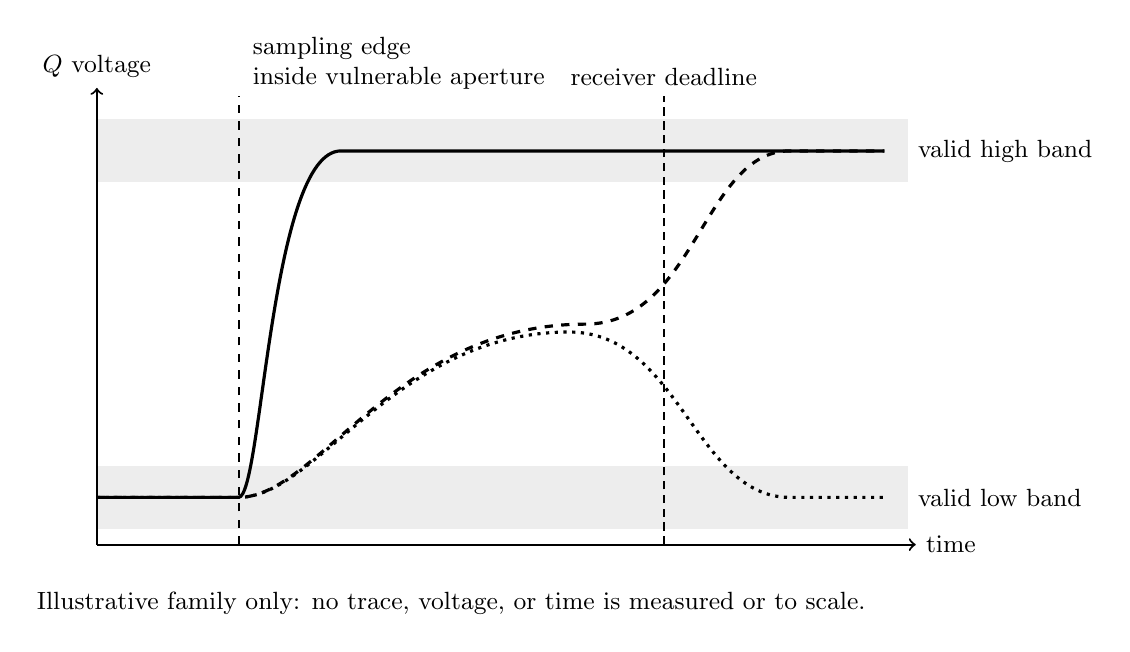
\begin{tikzpicture}[x=1cm,y=1cm,font=\small,line width=0.75pt,
  thick/.style={line width=1.15pt,line join=round}]
  \fill[gray!14] (1.2,4.9) rectangle (11.5,5.7);
  \fill[gray!14] (1.2,0.5) rectangle (11.5,1.3);
  \node[right] at (11.5,5.3) {valid high band};
  \node[right] at (11.5,0.9) {valid low band};
  \draw[->] (1.2,0.3) -- (11.6,0.3) node[right] {time};
  \draw[->] (1.2,0.3) -- (1.2,6.1) node[above] {$Q$ voltage};
  \draw[dashed] (3.0,0.3) -- (3.0,6.0);
  \node[above right,align=left] at (3.05,5.95)
    {sampling edge\\inside vulnerable aperture};
  \draw[densely dashed] (8.4,0.3) -- (8.4,6.0);
  \node[above,align=center] at (8.4,6.0) {receiver deadline};

  \draw[thick] (1.2,0.9) -- (3.0,0.9)
    .. controls (3.3,0.9) and (3.4,5.3) .. (4.3,5.3) -- (11.2,5.3);
  \draw[thick,dashed] (1.2,0.9) -- (3.0,0.9)
    .. controls (4.0,0.9) and (5.0,3.1) .. (7.4,3.1)
    .. controls (8.8,3.1) and (8.9,5.3) .. (10.0,5.3) -- (11.2,5.3);
  \draw[thick,dotted] (1.2,0.9) -- (3.0,0.9)
    .. controls (4.0,0.9) and (5.0,3.0) .. (7.2,3.0)
    .. controls (8.6,3.0) and (8.8,0.9) .. (10.0,0.9) -- (11.2,0.9);
  \node[align=center] at (5.7,-0.45)
    {Illustrative family only: no trace, voltage, or time is measured or to scale.};
\end{tikzpicture}
\end{document}
